\documentclass[12pt]{article}
\usepackage[margin=1in]{geometry}
\usepackage{listings}
\usepackage{graphicx}
\usepackage{float}
\usepackage{color} %red, green, blue, yellow, cyan, magenta, black, white
\definecolor{mygreen}{RGB}{28,172,0} % color values Red, Green, Blue
\definecolor{mylilas}{RGB}{170,55,241}

\setlength{\parskip}{1em}

\lstset{language=Matlab,%
    %basicstyle=\color{red},
    breaklines=true,%
    morekeywords={matlab2tikz},
    keywordstyle=\color{blue},%
    morekeywords=[2]{1}, keywordstyle=[2]{\color{black}},
    identifierstyle=\color{black},%
    stringstyle=\color{mylilas},
    commentstyle=\color{mygreen},%
    showstringspaces=false,%without this there will be a symbol in the places where there is a space
    numbers=left,%
    numberstyle={\tiny \color{black}},% size of the numbers
    numbersep=9pt, % this defines how far the numbers are from the text
    emph=[1]{for,end,break},emphstyle=[1]\color{red}, %some words to emphasise
    %emph=[2]{word1,word2}, emphstyle=[2]{style},    
}


\title{Assignment 1, COMP4702}
\author{Roy Portas}
\date{\today}

\begin{document}

\begin{titlepage}
    \maketitle
\end{titlepage}

\section*{Question 1.2}

The first column of the data is a timestamp, with each value being around 30 minutes apart. The data starts at the first of January 2015 and ends in the last day of December.

The second column appears to be a unique ID for each entry, as this number is never repeated and goes up by 1 for each record.

The third column contains numbers between 25 and 30, this is possibly a
temperature in degrees. The values also change gradually which seems correct for the given time intervals. 

Viewing data on the graph shows that the temperature is low at the start of the year and gradually climbs to it's max around 6 months in, then returns back to a lower temperature in December. This suggests that it is probably temperature measured in the northern hemisphere. Additionally this data has outliers, which is probably instrumentation error.

The fourth column contains numbers between 26 and around 50000. If this is plotted against the date, it can be seen that there are three distinct dips in the data. Two of the dips are at the start of the year and the last is towards the end.

The fifth column contains numbers between 7.3 and 8.3, with a mean of 7.846 and a standard StdDev of 0.142. This suggests that the value doesn't change much. Viewing the data over the date does not show any trends in the data.

When the sixth column is plotted against the fifth column, a linear relationship can be seen, as the values in the sixth column increases when the values of the fifth column increases. This indicates there is some form of relationship between two sets of data.

The last two columns don't provide much information, apart from increased outliers at the end of the year, suggesting that the sensors may be starting to fail.

It could possibly be weather data, containing temperature, humidity, etc.

\section*{Question 1.6}

\lstinputlisting[language=Matlab]{../../pracs/week2/q6.m}

\section*{Question 2.1}

\begin{figure}[H]
    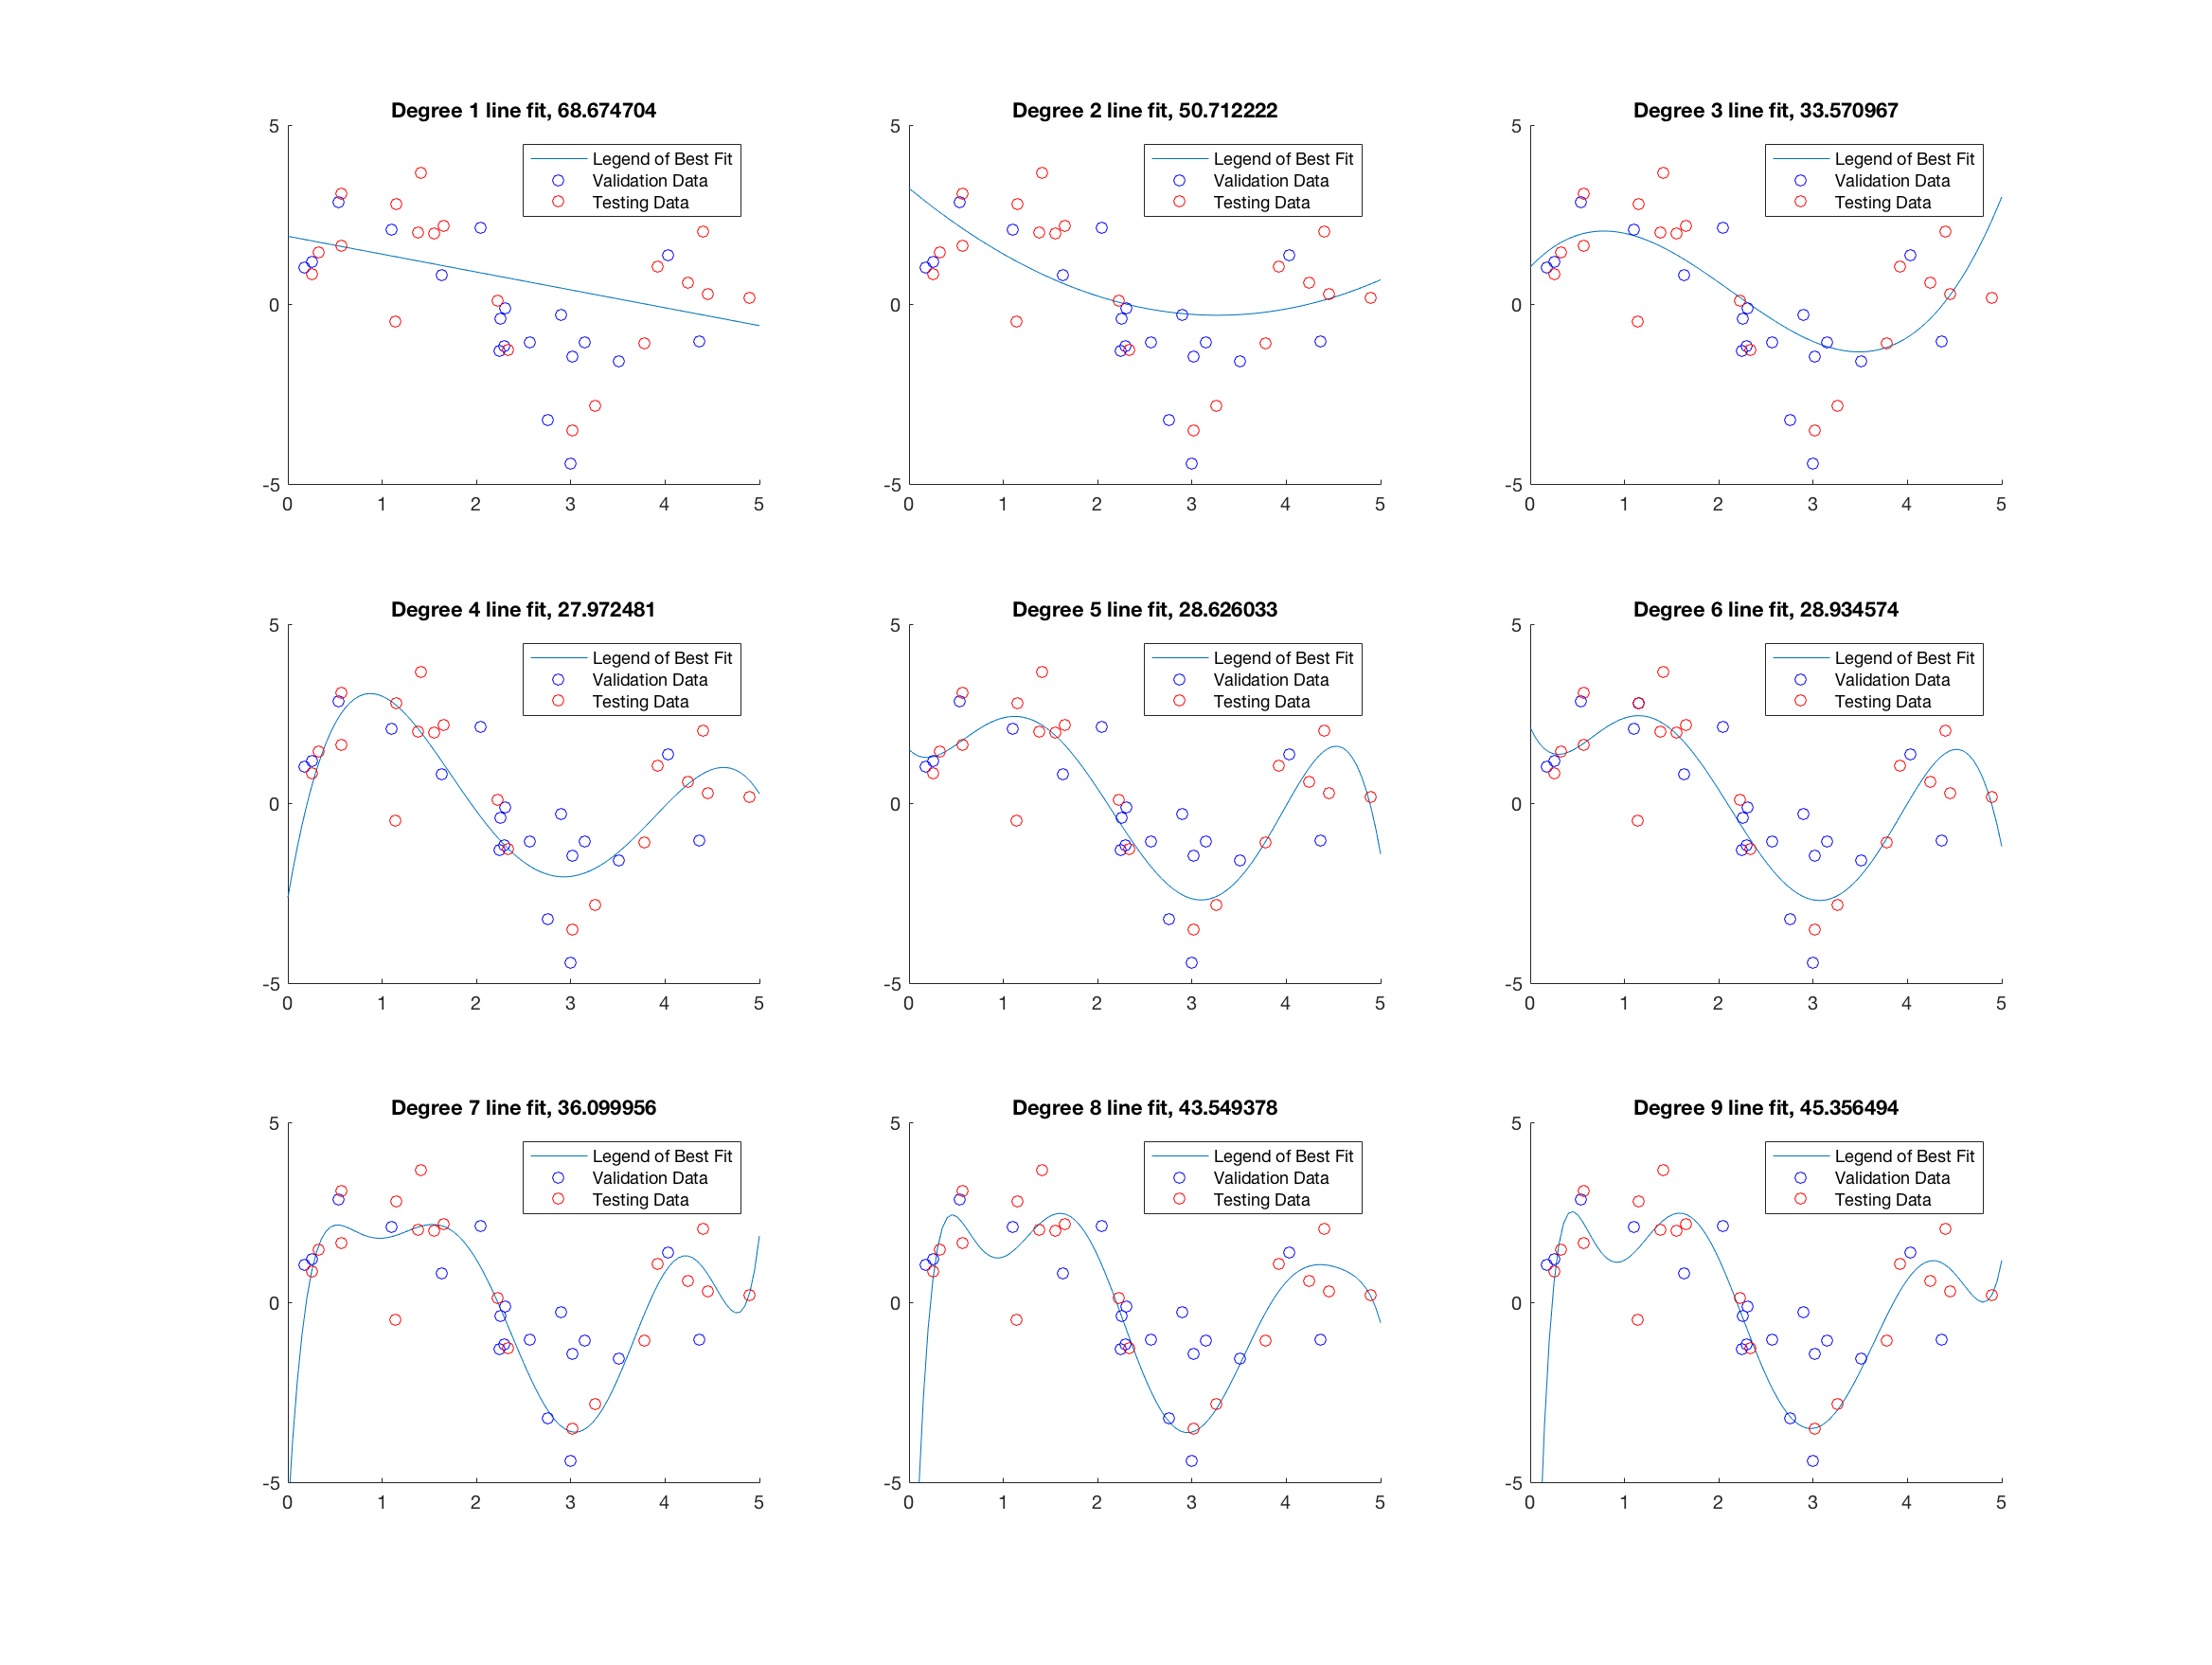
\includegraphics[width=\linewidth]{../../pracs/week3/images/q1_lines_of_best_fit}
    \centering
    \caption{Lines of best fit}
\end{figure}

\begin{figure}[H]
    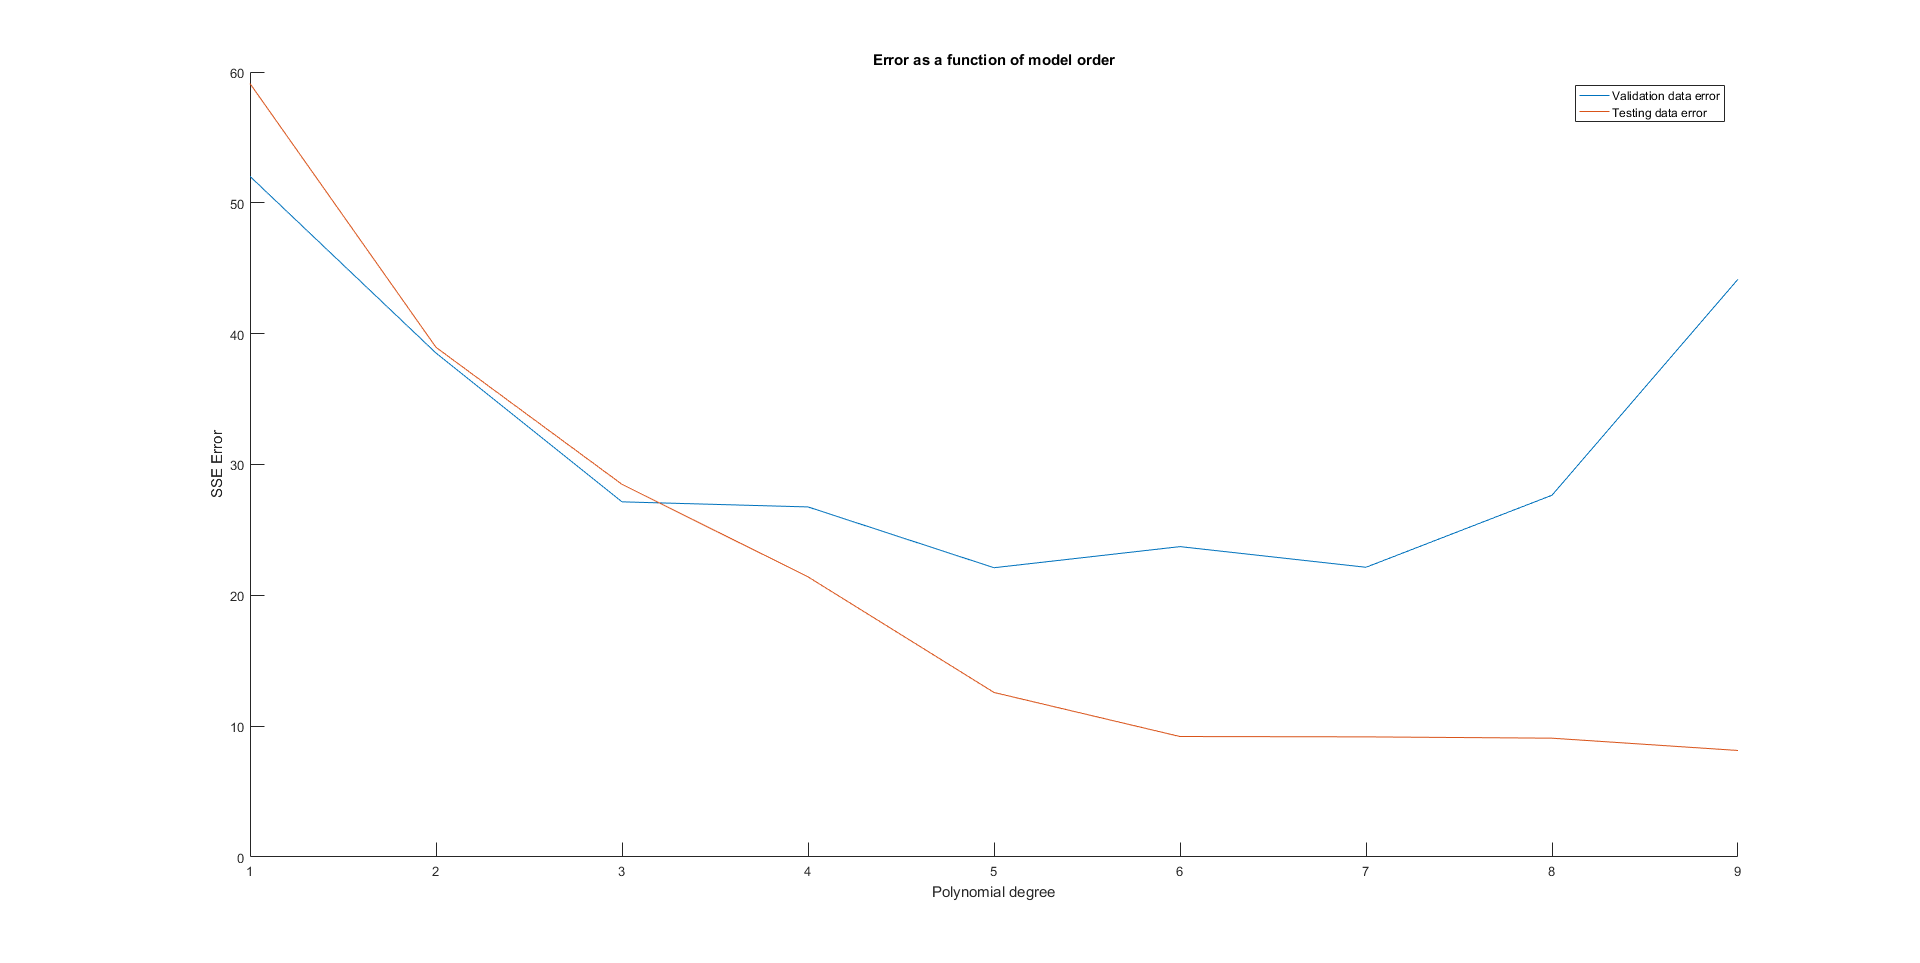
\includegraphics[width=\linewidth]{../../pracs/week3/images/q1_err_vs_degree}
    \centering
    \caption{Error vs Polynomial Degree}
\end{figure}

The above figure shows that as more polynomial degrees are introduced the error on the testing data decreases, which is expected as this was the data the model was trained on. However the error on the validation data increases after the 7th polynomial, thus we are overfitting the data.

\section*{Question 2.4}

\lstinputlisting[language=Matlab]{../../pracs/week3/q4.m}

\begin{figure}[H]
    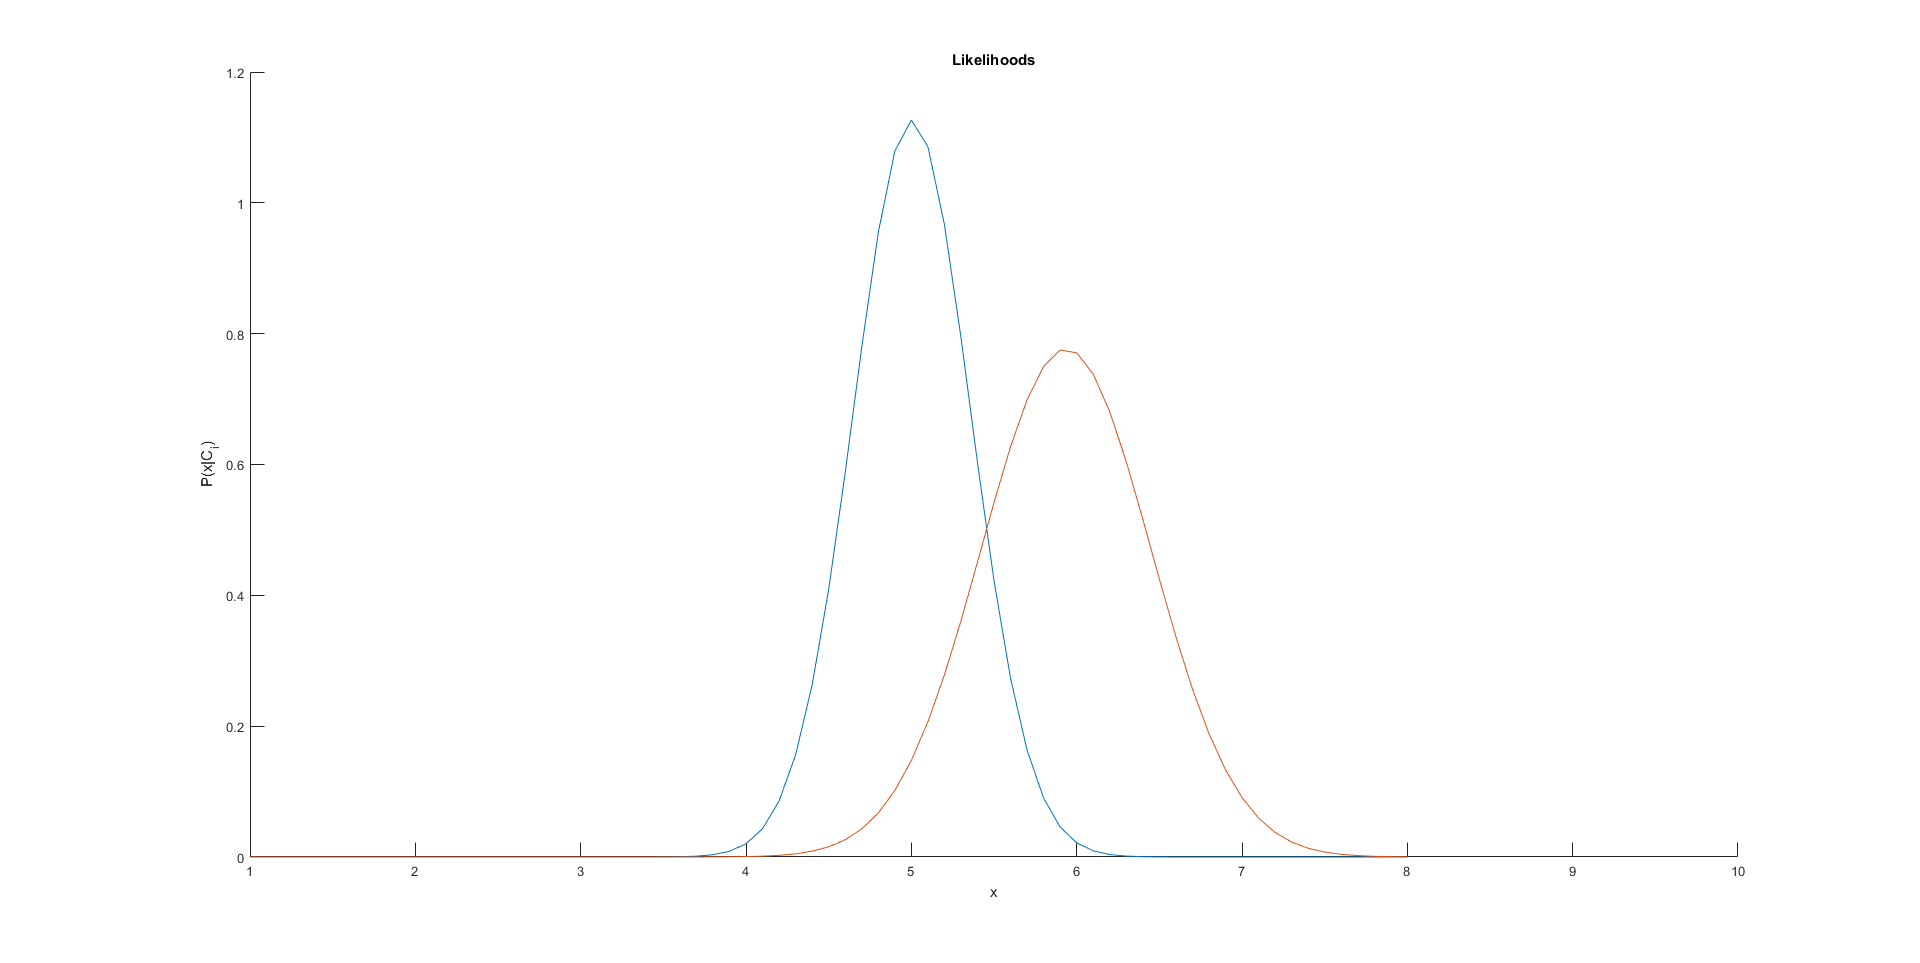
\includegraphics[width=\linewidth]{../../pracs/week3/images/q4_likelihoods}
    \centering
    \caption{Likelihoods}
\end{figure}

\begin{figure}[H]
    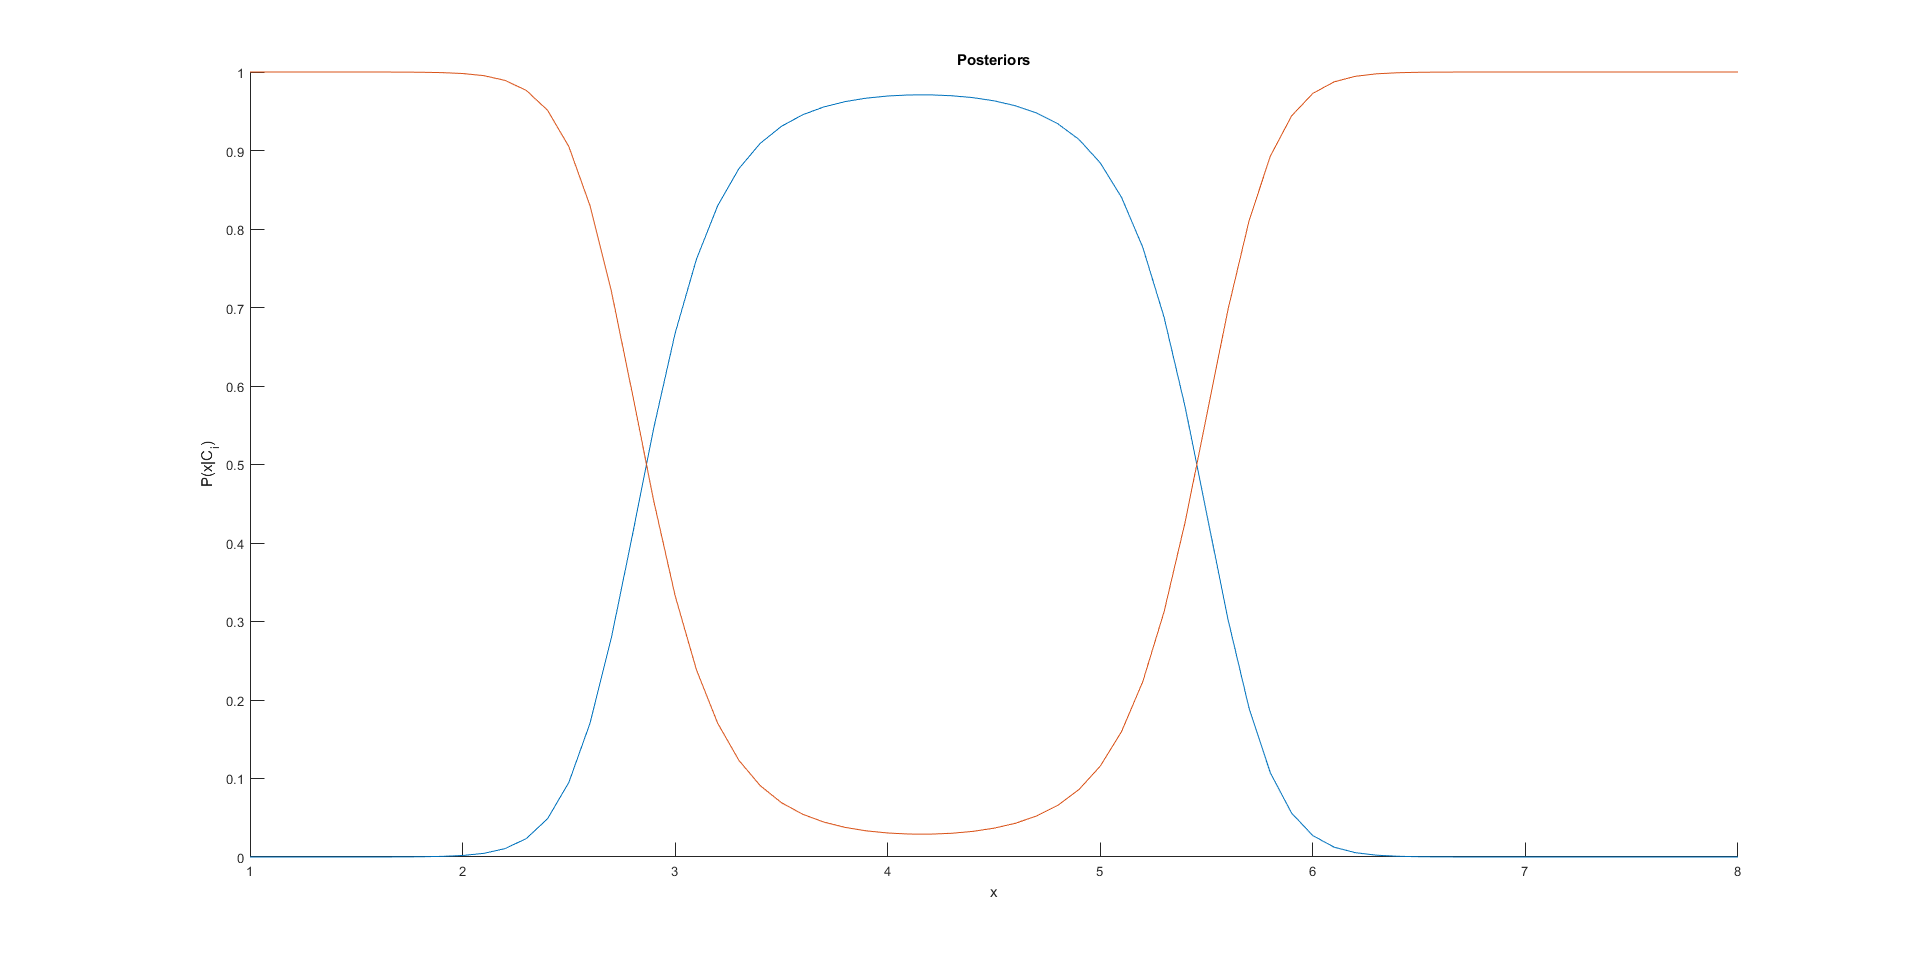
\includegraphics[width=\linewidth]{../../pracs/week3/images/q4_posteriors}
    \centering
    \caption{Posteriors}
\end{figure}

\section*{Question 3.1}

With the given dataset, we want to find a way to classify the two classes, this can be given by the posterior $P(C_i|x)$. To do so we first need to estimate the prior $P(C_i)$ and $p(x|C)$. This will allow us to estimate the proportion of data points for a given class $i$.  $p(x|c)$ can easily be found by using the matlab function \texttt{mvnpdf}.

Finding the posteriors for each class yields the below graph.

\begin{figure}[H]
    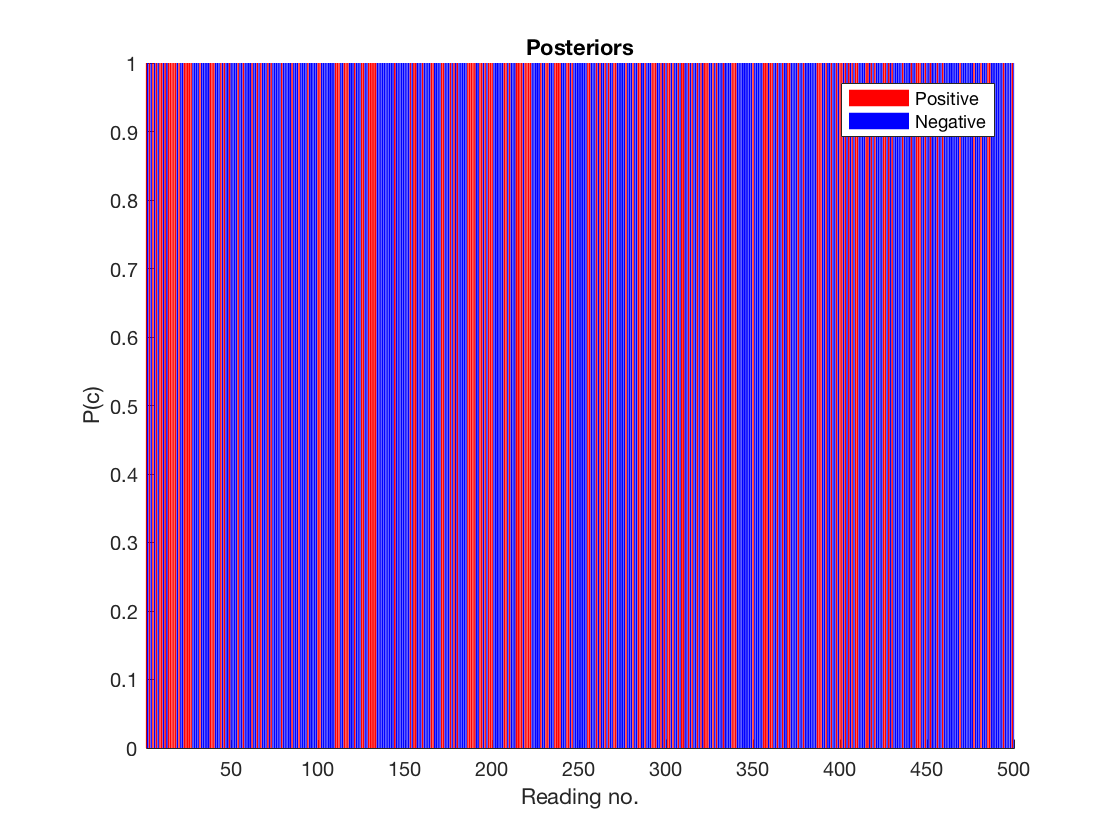
\includegraphics[width=\linewidth]{../../pracs/week4/images/q1_posteriors}
    \centering
    \caption{Posteriors}
\end{figure}

This shows the classification of the algorithm, visually we can see that there is more blue than red, meaning more people test negative to diabetes than positive, which makes sense when you look at the raw data.


The error on the training set was found to be $330.42$, while the error on the testing set was found to be $181.18$. This is possibly caused by the training set containing many more data rows than the testing set.

The model parameters were found to be the following:

\lstinputlisting[]{./q3-1-answer.txt}

\section*{Question 3.2}

LDA can be implemented similiar to the QDA done above.

\lstinputlisting[language=Matlab]{../../pracs/week4/q2.m}

The error for the training set was found to be $319.41$ and 
the error for the testing set was found to be $178.59$.

The model parameters are listed below

\lstinputlisting[]{./q3-2-answer.txt}

\section*{Question 3.5}

The computed KL values are listed in the table below
\begin{center}
    \begin{tabular}{|c|c|c|}
        \hline
        M and H1 & 2.6898 \\
        M and K1 & 0.2741  \\
        M and K2 & 0.28186 \\
        \hline
    \end{tabular}
\end{center}

There was an issue encountered while finding these variables, it was caused by the 0 values in some of the bins of the histogram estimator, this caused the division to produce Infinity values. This was fixed by replacing the infinity values with 0.

\begin{figure}[H]
    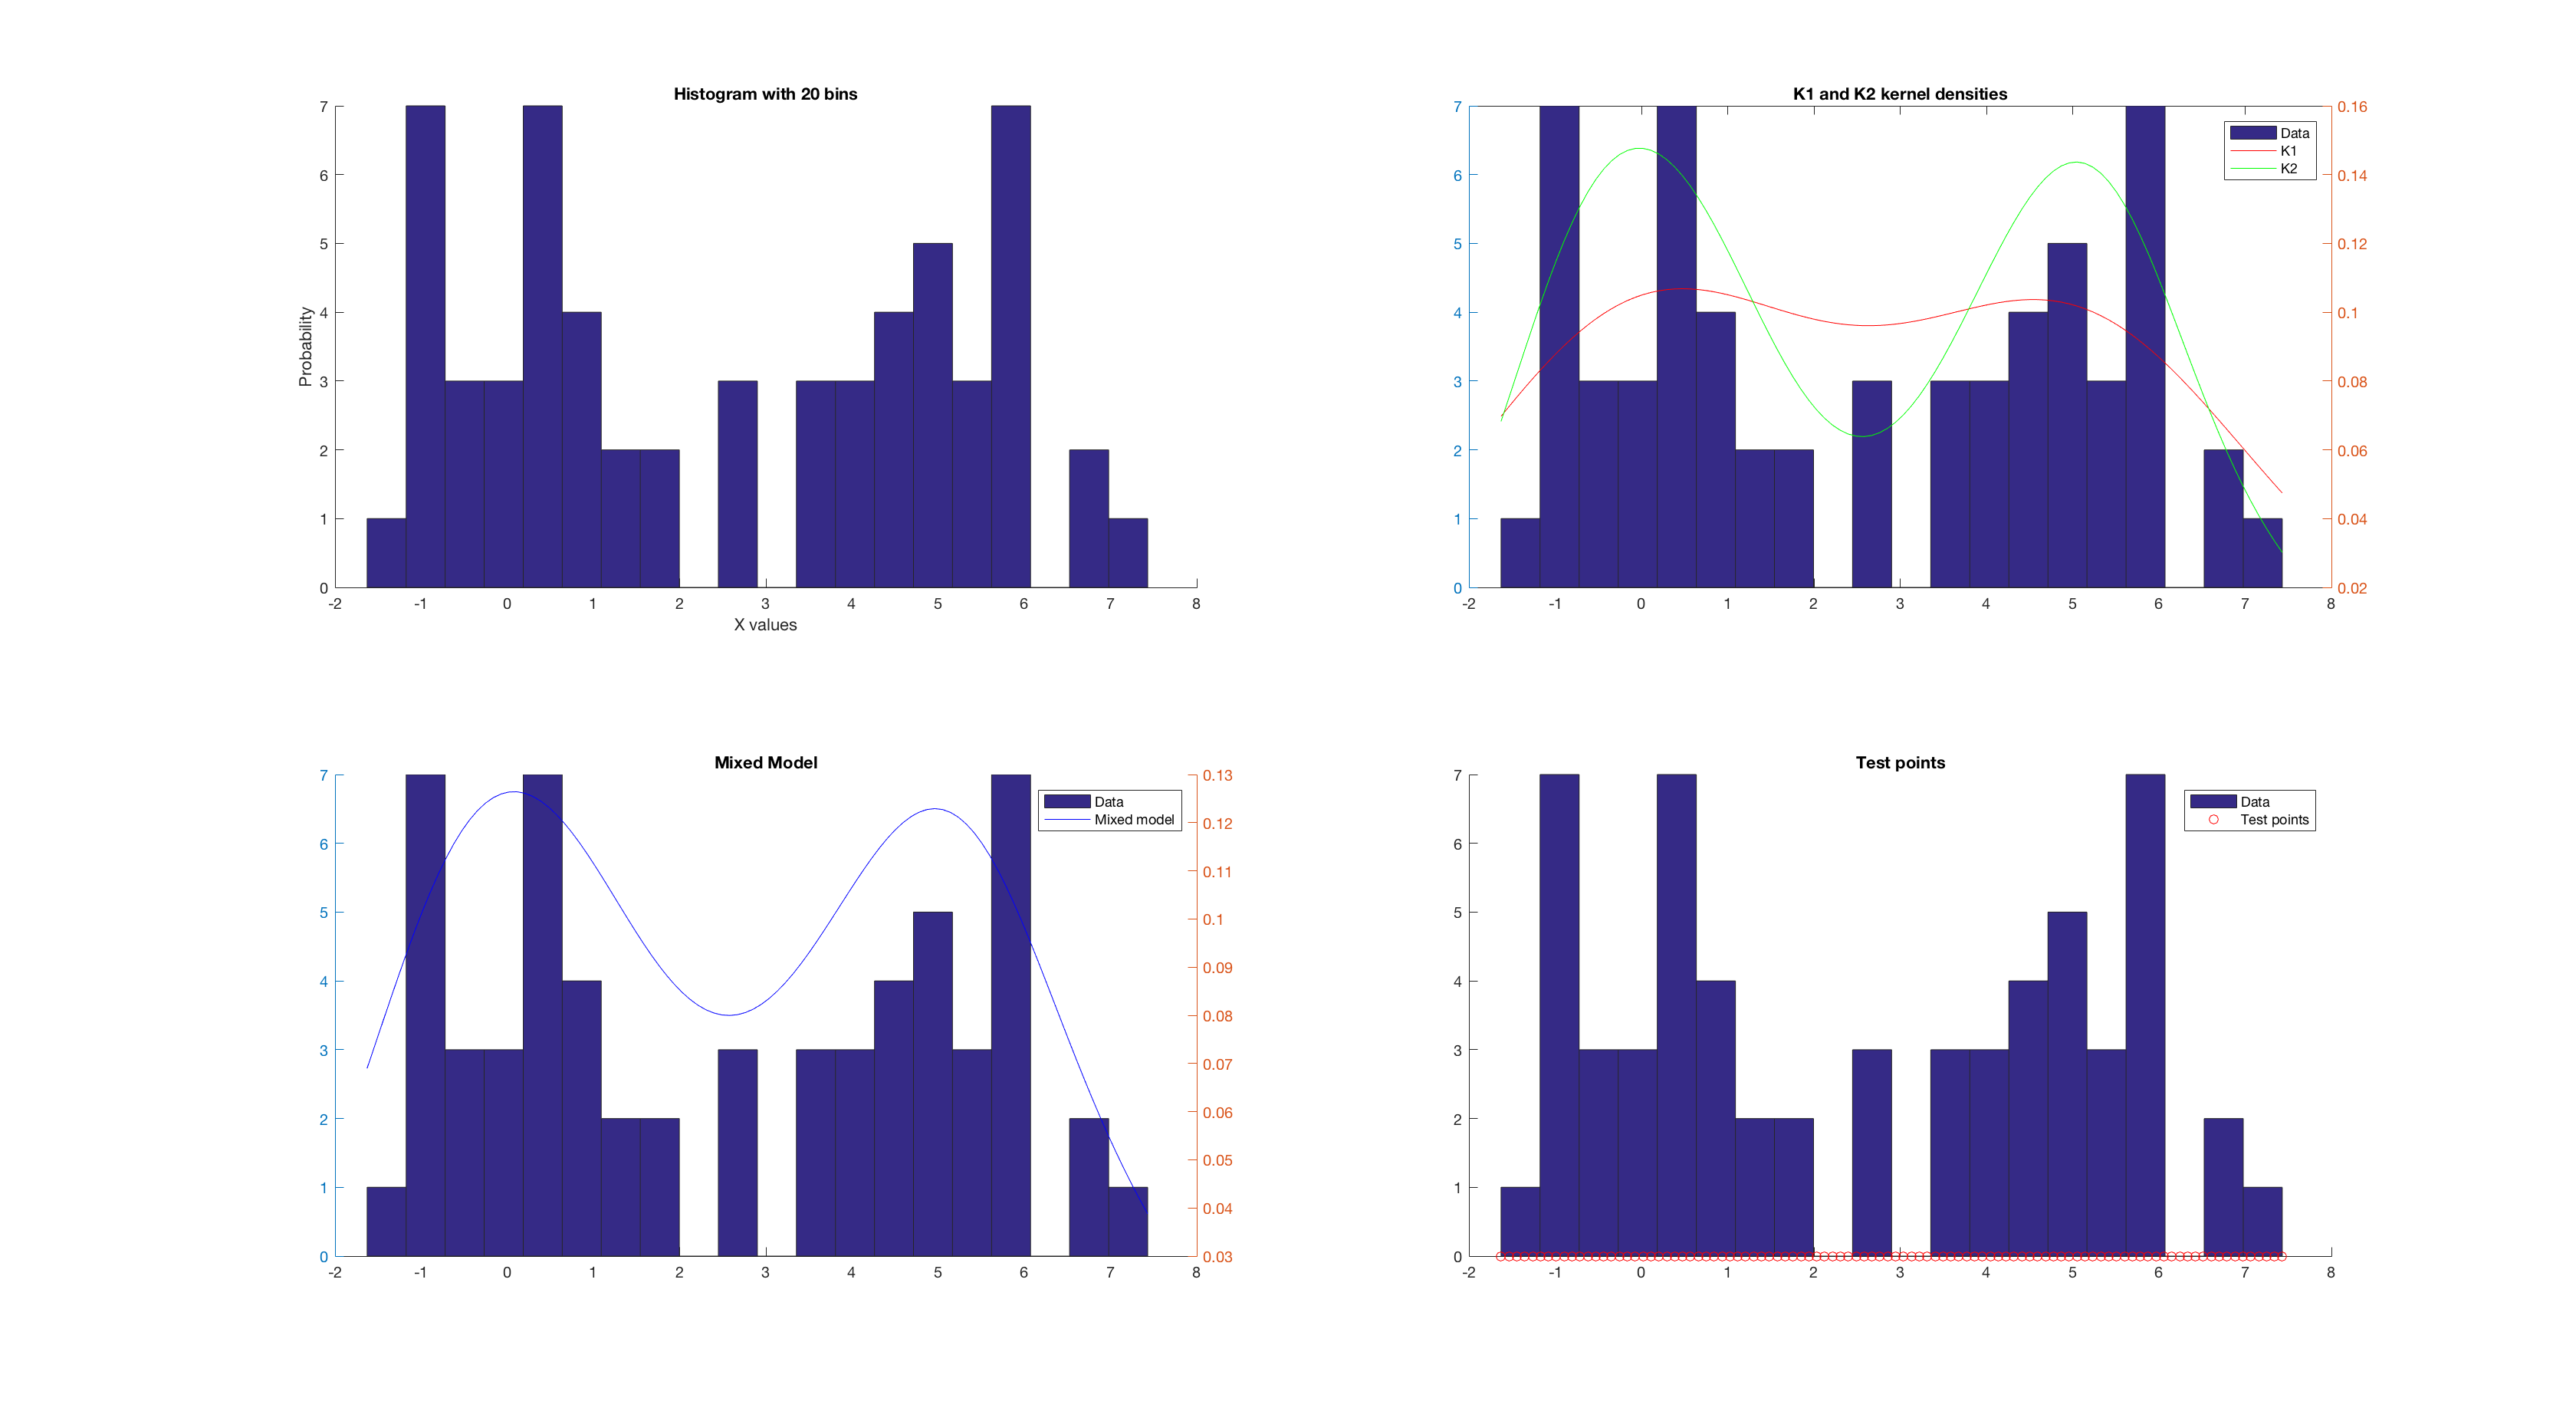
\includegraphics[width=\linewidth]{../../pracs/week4/images/q5}
    \centering
    \caption{Q5}
\end{figure}

Below is the code used to calculate the KL function, see the function called \texttt{KL} at the bottom of the script.

\lstinputlisting[language=Matlab]{../../pracs/week4/q5.m}

\end{document}
